\documentclass[12pt,hyperref,a4paper,UTF8]{ctexart}
\usepackage{HDUReport}
\usepackage{listings}
\usepackage{xcolor}
\usepackage{graphicx}
\usepackage{setspace}
\usepackage{float}
\setstretch{1.5} % 设置全局行距为1.5倍

\usepackage{enumitem} % 载入enumitem包以便自定义列表环境
\setlist[itemize]{itemsep=0pt, parsep=0pt} % 设置itemize环境的项目间距和段落间距

\setmainfont{Times New Roman} % 英文正文为Times New Roman


\usepackage{tikz}
\usetikzlibrary{shapes.geometric, arrows}
\usetikzlibrary{positioning, arrows.meta}
\usetikzlibrary{calc}


% 设置MATLAB代码样式
\definecolor{codegreen}{rgb}{0,0.6,0}
\definecolor{codegray}{rgb}{0.5,0.5,0.5}
\definecolor{codepurple}{rgb}{0.58,0,0.82}
\definecolor{backcolour}{rgb}{0.95,0.95,0.92}

\lstdefinestyle{matlab}{
    backgroundcolor=\color{backcolour},   
    commentstyle=\color{codegreen},
    keywordstyle=\color{magenta},
    numberstyle=\tiny\color{codegray},
    stringstyle=\color{codepurple},
    basicstyle=\ttfamily\small,
    breakatwhitespace=false,         
    breaklines=true,                 
    captionpos=b,                    
    keepspaces=true,                 
    numbers=left,                    
    numbersep=5pt,                  
    showspaces=false,                
    showstringspaces=false,
    showtabs=false,                  
    tabsize=2,
    frame=single,
    language=Matlab
}
%封面页设置
{   
    %标题
    \title{ 
        \vspace{1cm}
        \heiti \Huge \textbf{《数字信号处理课程设计》实验报告} \par
        \vspace{1cm} 
        \heiti \Large {\underline{实验报告2:FFT频谱分析}   } 
        \vspace{3cm}
    
    }

    \author{
        \vspace{0.5cm}
        \kaishu\Large 学院\ \dlmu[9cm]{卓越学院} \\ %学院
        \vspace{0.5cm}
        \kaishu\Large 学号\ \dlmu[9cm]{23040447} \\ %班级
        \vspace{0.5cm}
        \kaishu\Large 姓名\ \dlmu[9cm]{陈文轩} \qquad  \\ %学号
        \vspace{0.5cm}
        \kaishu\Large 专业\ \dlmu[9cm]{智能硬件与系统(电子信息工程)} \qquad \\ %姓名 
    }
        
    \date{\today} % 默认为今天的日期,可以注释掉不显示日期
}
%%------------------------document环境开始------------------------%%
\begin{document}

%%-----------------------封面--------------------%%
\cover
\thispagestyle{empty} % 首页不显示页码
%%------------------摘要-------------%%
%\newpage
%\begin{abstract}




%\end{abstract}

%\thispagestyle{empty} % 首页不显示页码

%%--------------------------目录页------------------------%%
% \newpage
% \tableofcontents
% \thispagestyle{empty} % 目录不显示页码

%%------------------------正文页从这里开始-------------------%
\newpage
\setcounter{page}{1} % 让页码从正文开始编号

%%可选择这里也放一个标题
%\begin{center}
%    \title{ \Huge \textbf{{标题}}}
%\end{center}
\section{实验目的}
1、通过这一实验,能够熟练掌握快速离散傅里叶变换(FFT)的原理及其用FFT进行频谱分析的基本方法。

2、在通过计算机上用软件实现 FFT 及信号的频谱分析。

3、通过实验对离散傅里叶变换的主要性质及 FFT在数字信号处理中的重要作用有进一步的了解。

\section{实验基本原理}

\subsection{快速傅里叶变换(FFT)基本原理}

离散傅里叶变换(DFT)是将时域离散信号变换到频域的一种基本方法,其定义为:
\begin{equation}
X[k] = \sum_{n=0}^{N-1} x[n]e^{-j\frac{2\pi}{N}kn}, \quad k = 0,1,\ldots,N-1
\end{equation}

其逆变换(IDFT)定义为:
\begin{equation}
x[n] = \frac{1}{N}\sum_{k=0}^{N-1} X[k]e^{j\frac{2\pi}{N}kn}, \quad n = 0,1,\ldots,N-1
\end{equation}

直接计算DFT需要$O(N^2)$的计算复杂度。快速傅里叶变换(FFT)通过分解算法,将计算复杂度降至$O(N\log_2 N)$,显著提高了计算效率。

\subsubsection{基2FFT算法(Cooley-Tukey算法)}
基2FFT算法基于序列长度为2的整数幂($N=2^m$)时,可将DFT分解为更小规模的DFT计算。具体地,将序列分为奇偶两组:
\begin{equation}
X[k] = \sum_{r=0}^{N/2-1} x[2r]e^{-j\frac{2\pi}{N}k(2r)} + \sum_{r=0}^{N/2-1} x[2r+1]e^{-j\frac{2\pi}{N}k(2r+1)}
\end{equation}

令$W_N = e^{-j\frac{2\pi}{N}}$,上式可重写为:
\begin{equation}
X[k] = \sum_{r=0}^{N/2-1} x[2r]W_N^{2rk} + W_N^k\sum_{r=0}^{N/2-1} x[2r+1]W_N^{2rk}
\end{equation}

注意到$W_N^2 = W_{N/2}$,可得:
\begin{equation}
X[k] = G[k] + W_N^k \cdot H[k]
\end{equation}
其中$G[k]$和$H[k]$分别是偶序列和奇序列的DFT,各自长度为$N/2$。

由于$G[k]$和$H[k]$的周期性,对于$k+N/2$:
\begin{equation}
X[k+N/2] = G[k] - W_N^k \cdot H[k]
\end{equation}

这种蝶形运算结构可递归应用,直至最小规模的DFT(N=2)。

\subsection{FFT频谱分析原理}

频谱分析是分析信号频率成分的方法,通过FFT可以高效计算信号的频谱。对于长度为N的序列,其频谱分析过程如下:

\subsubsection{频谱计算}
通过FFT计算信号的频域表示:
\begin{equation}
X[k] = \text{FFT}(x[n]), \quad k = 0,1,\ldots,N-1
\end{equation}

\subsubsection{频率分辨率}
对于采样频率为$f_s$的信号,频率分辨率为:
\begin{equation}
\Delta f = \frac{f_s}{N}
\end{equation}
第$k$个频点对应的实际频率为:$f_k = k \cdot \Delta f$(对于$0 \leq k \leq N/2$)。

\subsubsection{功率谱计算}
信号的功率谱密度(PSD)可通过以下方式计算:
\begin{equation}
P[k] = \frac{|X[k]|^2}{N}, \quad k = 0,1,\ldots,N-1
\end{equation}

对于单边谱,需要对$k=1,2,\ldots,N/2-1$的值乘以2(因为对称性)。

\section{实验要求及内容}


(1) 周期为 N 的正弦序列 \(\sin(\frac{2\pi}{N}n)\),且 \(0\leq n\leq N-1\),N=32,求 N 点 DFT。

(2) 复合函数序列 \(0.9\sin(\frac{2\pi}{N}n) + 0.6\sin(\frac{2\pi}{N/3}n)\)

(3) 矩形序列 \(R_N(n)\) ,N=8;求 N 点 DFT 和 2N 点 DFT。

(4) 见教材习题 2.31

有一调幅信号
\begin{align*}
x_\alpha(t) = [1 + \cos(2\pi \times 100t)] \cos(2\pi \times 600t)
\end{align*}

DFT  做频谱分析,要求能分辨 \(x_q(t)\) 的所有频率分量,若用 \(f_x = 3kHz\) 频率抽样,首先分析抽样数据为 N=120 点的频谱分析,求 \(X(k) = DFT[x(n)]\),N=120 点,画出 \(X(k)\) 的幅频特性 \(\left|X(k)\right|\),标出主要点的坐标值。其次分析抽样数据为 N=128 点的频谱分析,求 \(X(k) = DFT[x(n)]\),N=128 点,画出 \(X(k)\) 的幅频特性 \(\left|X(k)\right|\),标出主要点的坐标值。

比较上述不同长度采样点情况下的实验结果,说明利用 DFT 对连续信号进行傅里叶分析可能造成哪些误差?






\section{实验结果与分析}

\subsection{题目一}


% 插入MATLAB代码
\begin{lstlisting}[style=matlab, caption={实验一MATLAB实现代码}]
clear all
N = 32;
n = 0:N-1;
xn = sin(2*pi*n/N)  %32点的正弦信号 
XK = fft(xn, N);   %32点FFT转换
magXK = abs(XK);
phaXK = angle(XK);

subplot(1,2,1)
plot(n, xn)
xlabel('n'); ylabel('x(n)');
title('x(n) N=32');

subplot(1,2,2)
k = 0:length(magXK)-1;  %绘制时域信号和频域幅度谱
stem(k, magXK, '.'); 
xlabel('k'); ylabel('|X(k)|');
title('X(k) N=32');


%频谱特性解释:
%频点横坐标确定:生成的信号是频率为1周期/32点的正弦波,在DFT后,理论上应该在k=1和k=31(即N-1)处有两个峰值
                %这是因为DFT的周期性:k=N-1对应的是负频率分量(-1/32点),K=1对应的是正频率分量(1/32点)
                %正负频率分量,关于N/2对称,这是FFT频谱的特性
%频点强度确定:对于纯正弦波Asin(2πfn),DFT系数的理论幅度为AN/2,这里就是16
\end{lstlisting}



\begin{figure}[H] % [H] 表示强制当前位置插入
        \centering
        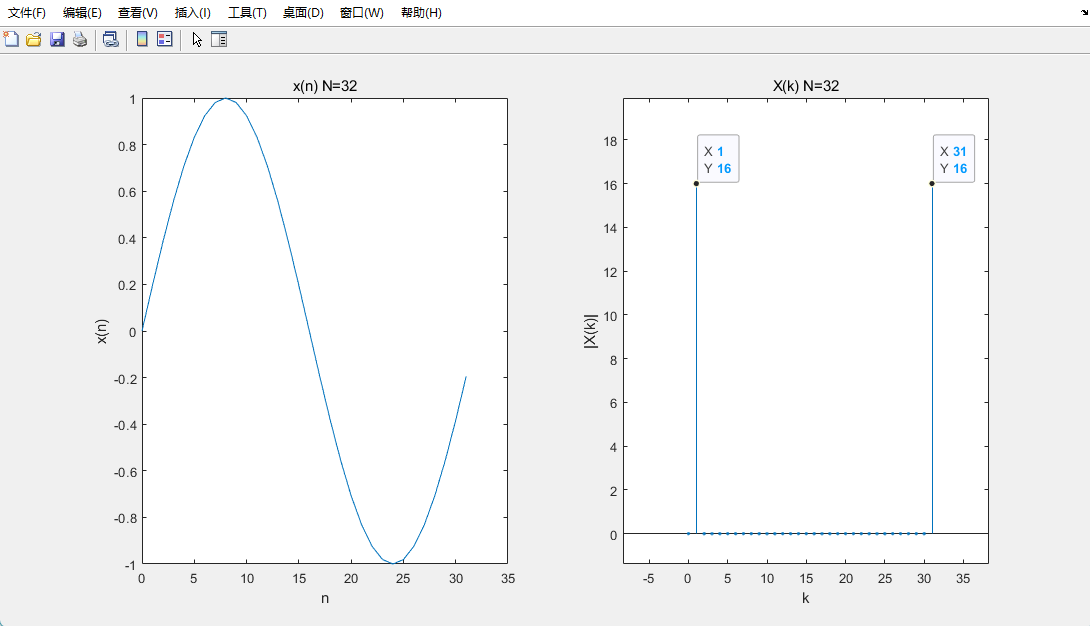
\includegraphics[width=0.9\textwidth]{figures/301.png} % 调整宽度为文本宽度的 80%
        \caption{matlab绘图} %图片标题
        \label{fig:example} % 图片标签,用于引用
\end{figure}



\subsection{题目二}


% 插入MATLAB代码
\begin{lstlisting}[style=matlab, caption={ MATLAB实现代码}]
clear all
N = 100;
n = 0:N-1;
xn = 0.9*sin(2*pi*n/N) + 0.6*sin(2*pi*n/N*3);
%时域信号构成:
%第一个正弦波:频率1周期/100点,幅度0.9
%第二个正弦波:频率3周期/100点,幅度0.6

XK = fft(xn, N);
magXK = abs(XK);
phaXK = angle(XK);

subplot(1,2,1)
plot(n, xn)
xlabel('n'); ylabel('x(n)');
title('x(n) N=100');

subplot(1,2,2)
k = 0:length(magXK)-1; %绘制时域信号和频域幅度谱
stem(k, magXK, '.'); 
xlabel('k'); ylabel('|X(k)|');
title('X(k) N=100');

%FFT频谱解释:
%横坐标(k):DFT频点序号(0到99)
    %k=1对应频率:1/100 cycles/sample(即第一个正弦波)
    %k=3对应频率:3/100 cycles/sample(即第二个正弦波)
    %k=97对应频率:-3/100 cycles/sample(第二个正弦波的负频率分量)
    %k=99对应频率:-1/100 cycles/sample(第一个正弦波的负频率分量)    
    %正负频率分量关于N/2对称
%纵坐标(|X(k)|):频谱幅度(理论预测值)
    %对于幅度A的正弦波,DFT峰值幅度应为A*N/2
    %第一个正弦波:0.9×100/2 = 45(k=1和k=99)
    %第二个正弦波:0.6×100/2 = 30(k=3和k=97)

%由于 N=3 太小,无法分辨原始信号中的高频分量(3 cycles/100),导致频谱严重失真。
%当 N=3,最高可分辨频率是 0.5 cycles/sample(Nyquist 频率)。但原信号的高频分量0.03cycles/sample 在 N=3 时被 混叠(aliasing) 到低频。
%原信号周期100/3=33.3,N=3太短,频谱泄漏严重
\end{lstlisting}



\begin{figure}[H] % [H] 表示强制当前位置插入
        \centering
        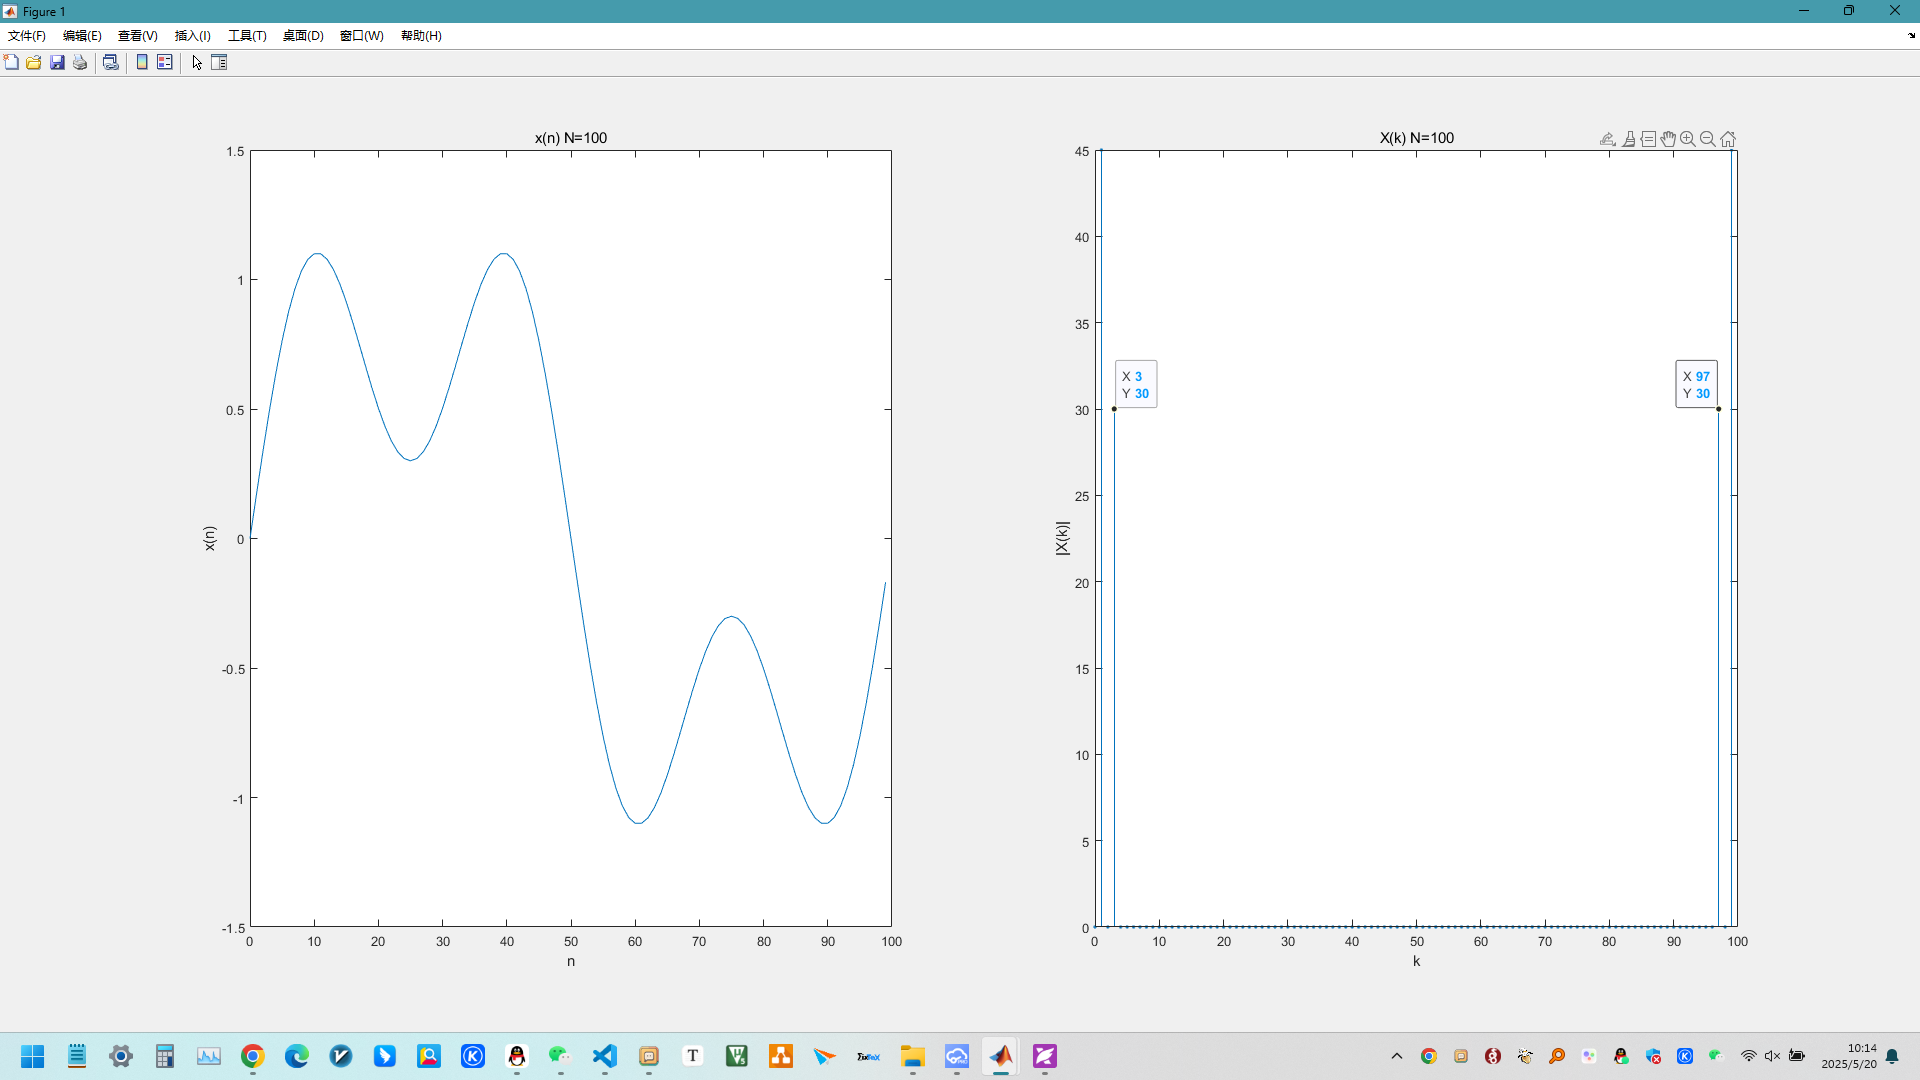
\includegraphics[width=0.9\textwidth]{figures/302.png} % 调整宽度为文本宽度的 80%
        \caption{matlab绘图} %图片标题
        \label{fig:example} % 图片标签,用于引用
\end{figure}


\subsection{题目三}


% 插入MATLAB代码
\begin{lstlisting}[style=matlab, caption={ MATLAB实现代码}]
clear all
M = 16;
n=[0:1:7];
N = length(n);
xn = ones(1,N);   %这是一个宽度为8的矩形脉冲,在数字信号处理中称为矩形窗函数
X1K = fft(xn, N); %FFT运算
X2K = fft(xn, M);
magX1K = abs(X1K);
phaX1K = angle(X1K);
magX2K = abs(X2K);
phaX2K = angle(X2K);

subplot(1,3,1)
stem(n, xn)
xlabel('n'); ylabel('x(n)');
title('x(n) N=8');

subplot(1,3,2)
k1 = 0:length(magX1K)-1; % Corrected the index calculation
stem(k1, magX1K, '.'); % Changed '.' to '.' for marker style
xlabel('k'); ylabel('|X(k)|');
title('X(k) N=8');

subplot(1,3,3)
k2 = 0:length(magX2K)-1; % Corrected the index calculation
stem(k2, magX2K, '.'); % Changed '.' to '.' for marker style
xlabel('k'); ylabel('|X(k)|');
title('X(k) M=16');

%频谱图1:(N=8)
%FFT分析:对8点信号做8点FFT(N=8)
%对于8点采集宽度为8的矩形脉冲,就是只有直流信号(时域信号幅值一直为1,没有振荡成分,没有交流分量)
%所以K=1~7(交流分量)FFT频谱上的幅值就是0,所有FFT幅值都在k=0
%k=0,e^j0=1,计算得幅值为8

%频谱图2:(N=16)
%幅值:对于16点采集宽度为8的矩形脉冲,时域呈现出窗函数,窗函数对应的FFT频谱就是离散Sinc函数,并关于N/2对称
%横坐标:由于分子1-e^(j*pi*k)为偶数时为 0,奇数时为 2,所以奇数时有幅值,偶数时没有幅值,而是呈现离散 sinc 函数的形状。
\end{lstlisting}



\begin{figure}[H] % [H] 表示强制当前位置插入
        \centering
        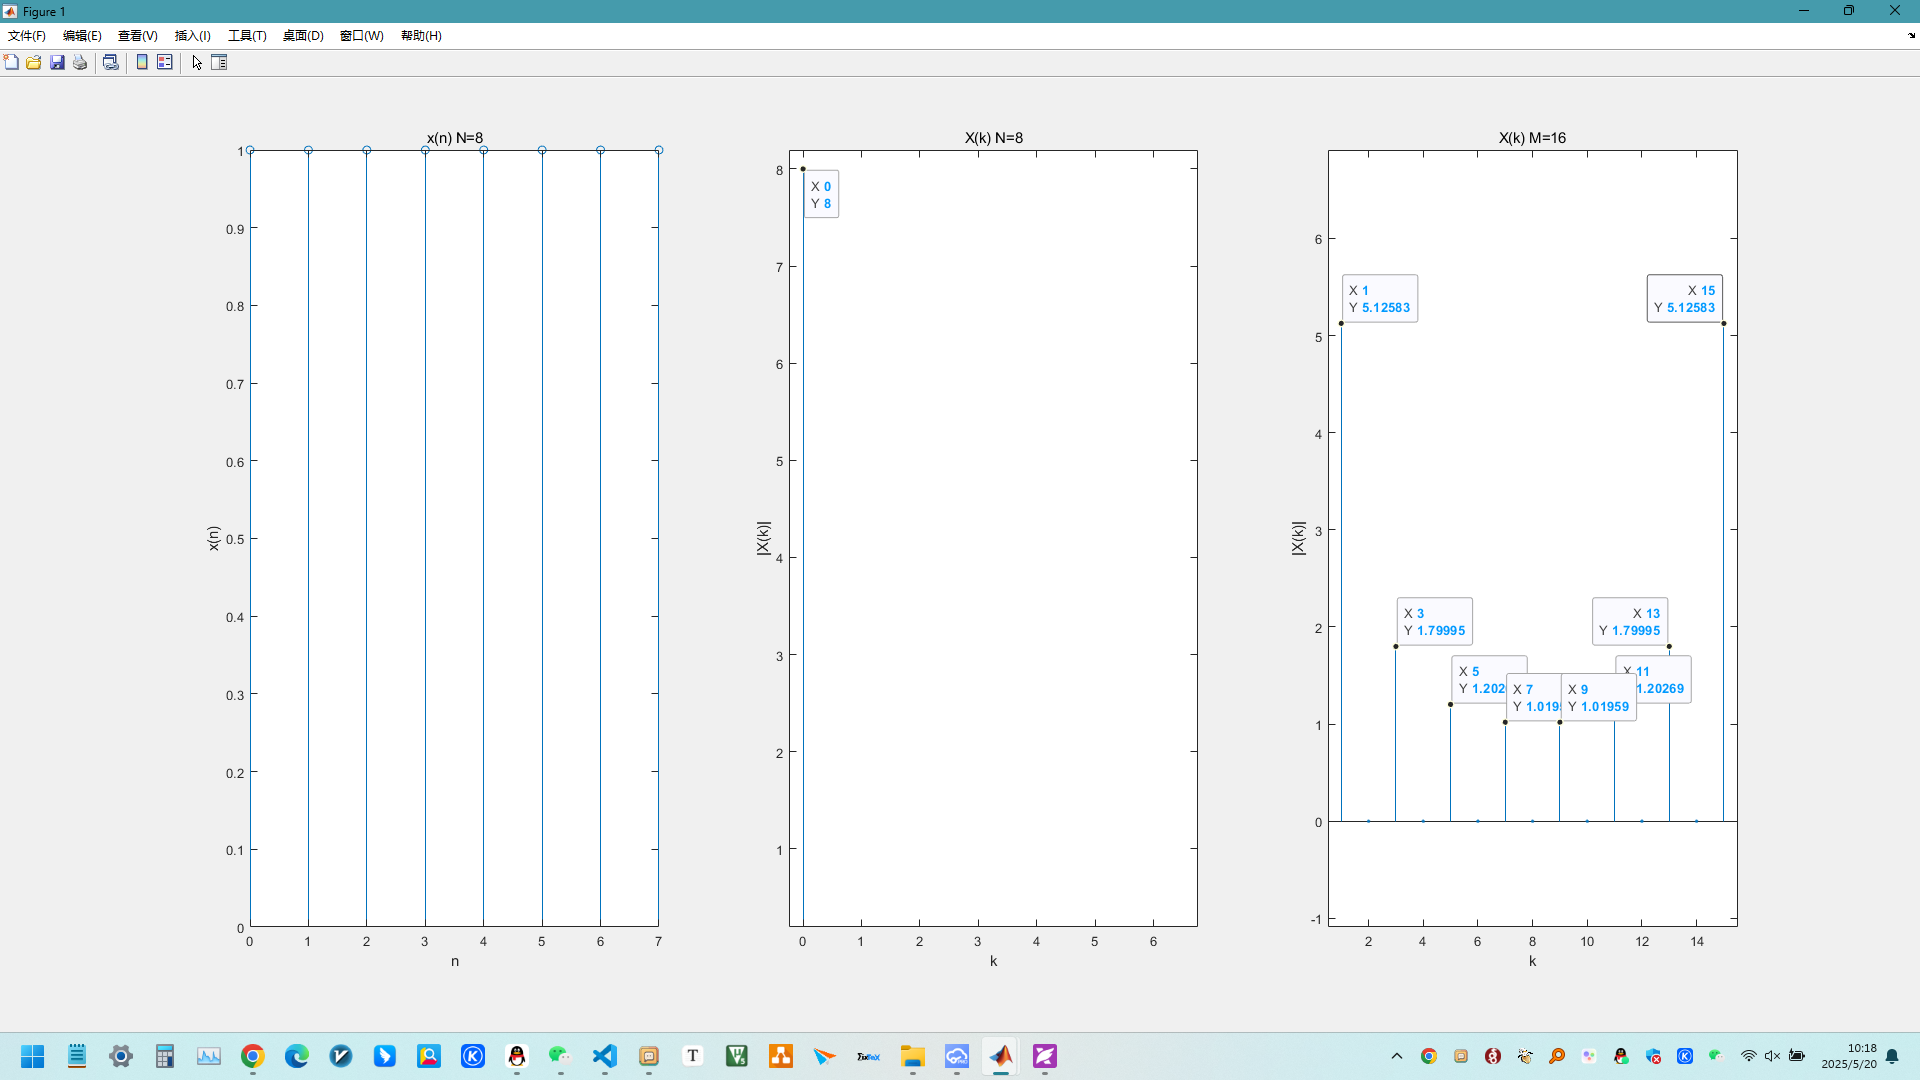
\includegraphics[width=0.9\textwidth]{figures/303.png} % 调整宽度为文本宽度的 80%
        \caption{matlab绘图} %图片标题
        \label{fig:example} % 图片标签,用于引用
\end{figure}


\subsection{题目四}


% 插入MATLAB代码
\begin{lstlisting}[style=matlab, caption={ MATLAB实现代码}]
clear all
N = 128;
M = 120;
fs = 3000 ;
t=0:1/fs:120/3000;  %采样时间40ms,整数周期采样
t2=0:1/fs:128/3000;  %采样时间42.67ms,非整数周期采样

xn = cos(2*pi*600*t).*(1+cos(2*pi*100*t));
x2n = cos(2*pi*600*t2).*(1+cos(2*pi*100*t2));
%这是一个幅度调制信号:
%载波:600 Hz 余弦波(高频)。
%调制信号:100 Hz 余弦波(低频),叠加直流分量1,形成时变幅度。

%FFT频谱解释:
%N=120:
%频率分辨率:Fs/120=25HZ
%AM时域信号积化和差得:x(t)=cos(2pai*600t)+0.5*cos(2pai*500t)+0.5*cos(2pai*700t)
%所以横坐标在k=20,24,28有幅值,且k=24的幅值为其余两个的两倍
%对于单频余弦信号,FFT频谱幅值为AN/2,所以k=20时,幅值就是0.5*120/2=30

%N=128
%频率分辨率:Fs/128=23.44HZ
%频谱出现能量扩散(频谱泄漏),因为信号频率未对齐DFT频点。
%主峰(600 Hz,k=25.6(无法对应))和边带(500/700 Hz)的能量会分散到多个频点。

XK = fft(x2n, N); %N=120采样
X1K = fft(xn, M);
magXK = abs(XK);
phaXK = angle(XK);

magX1K = abs(X1K);
phaX1K = angle(X1K);


subplot(1,4,1)
plot(t, xn)
xlabel('n'); ylabel('x(n)');
title('x(n) N=120');

subplot(1,4,2)
plot(t2, x2n)
xlabel('n'); ylabel('x(n)');
title('x(n) N=128');

subplot(1,4,3)
k = 0:length(magXK)-1; % Corrected the index calculation
stem(k, magXK, '.'); % Changed '.' to '.' for marker style
xlabel('k'); ylabel('|X(k)|');
title('X(k) N=128');

subplot(1,4,4)
k1 = 0:length(magX1K)-1; % Corrected the index calculation
stem(k1, magX1K, '.'); % Changed '.' to '.' for marker style
xlabel('k'); ylabel('|X(k)|');
title('X(k) N=120');



\end{lstlisting}



\begin{figure}[H] % [H] 表示强制当前位置插入
        \centering
        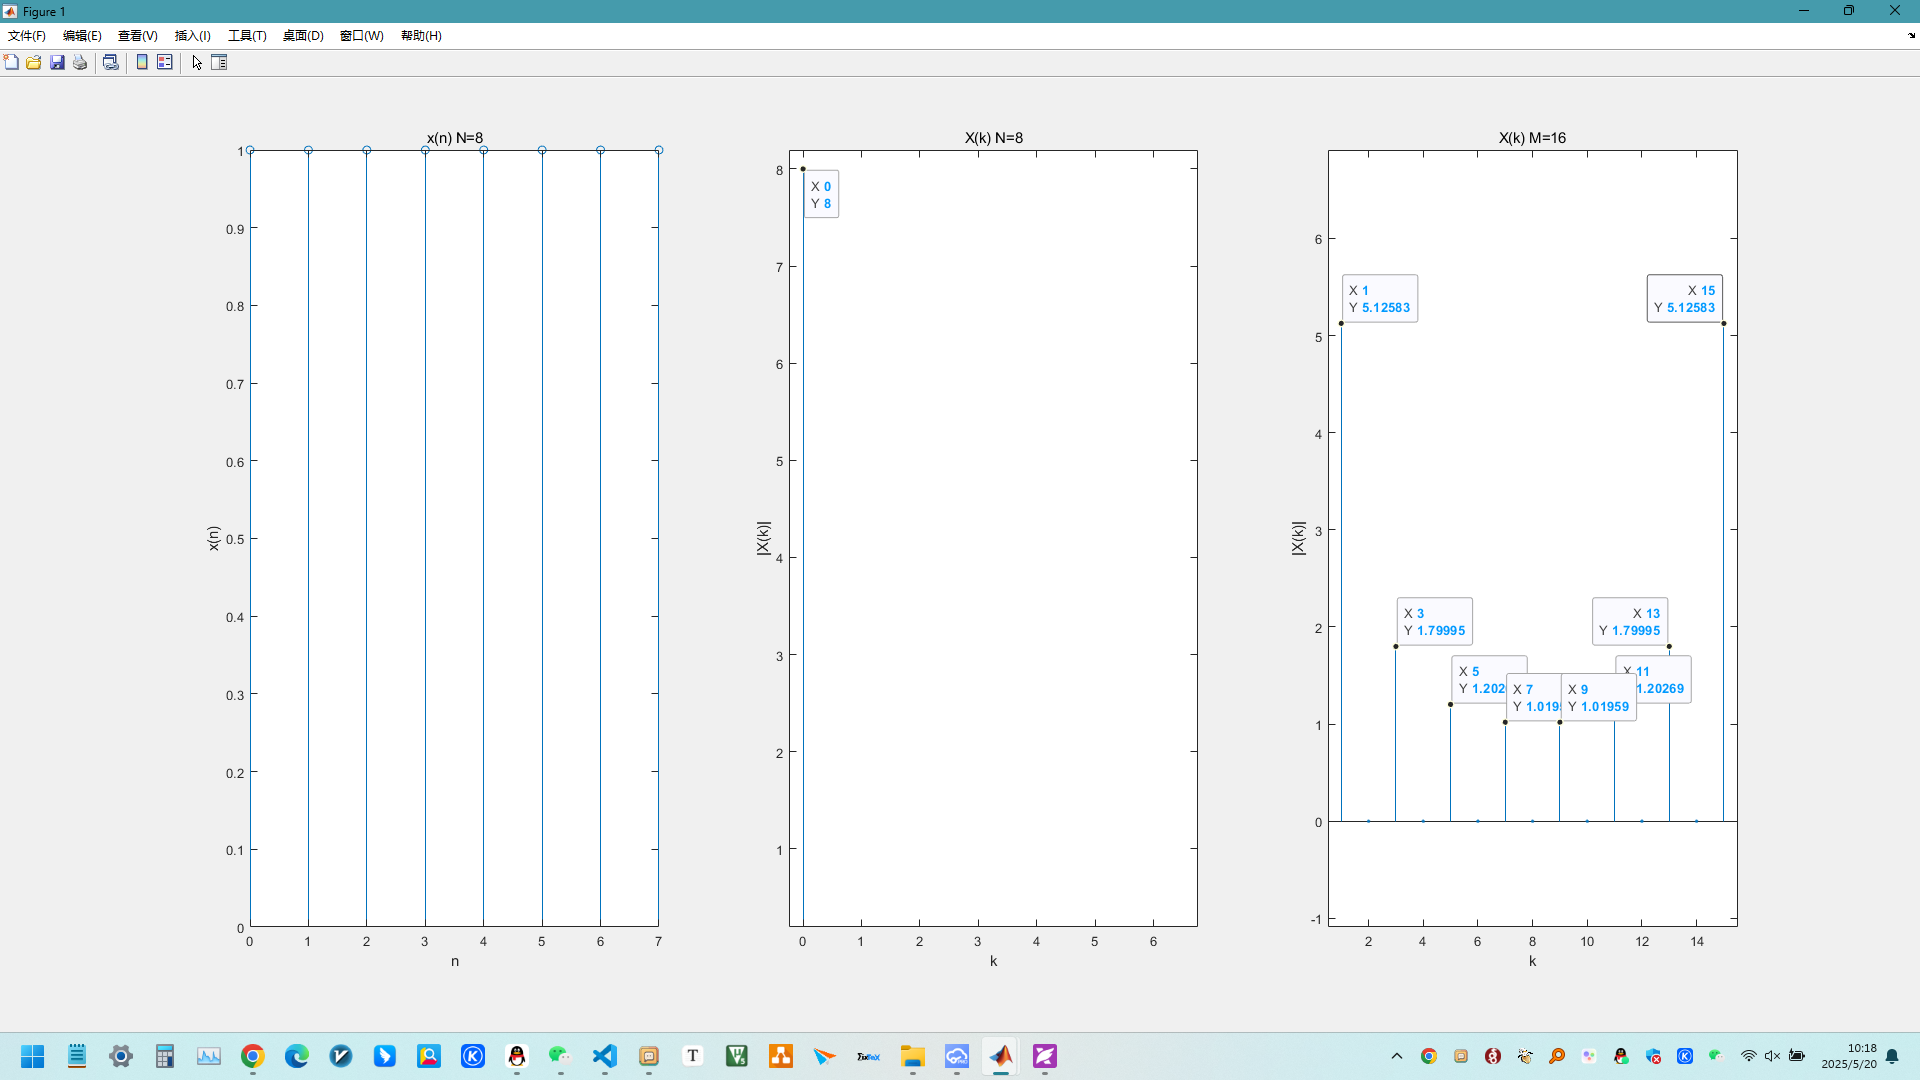
\includegraphics[width=0.9\textwidth]{figures/304.png} % 调整宽度为文本宽度的 80%
        \caption{matlab绘图} %图片标题
        \label{fig:example} % 图片标签,用于引用
\end{figure}

\section{实验小结}

通过本次快速傅里叶变换(FFT)频谱分析实验,我系统地学习了FFT算法的基本原理和应用技巧,掌握了在MATLAB环境下进行频谱分析的方法。通过四个不同的实验案例,我对FFT分析的特性有了更加深入的理解:

\subsection{关键发现}

\begin{enumerate}
    \item \textbf{FFT的基本特性}:通过实验一和二,验证了单频和多频信号的FFT频谱特性。对于频率为$f=1/N$的正弦信号,其频谱在$k=1$和$k=N-1$处呈现对称峰值,幅值理论上为$AN/2$,这与实验结果相符。
    
    \item \textbf{频谱泄漏现象}:在实验四中,通过比较N=120和N=128点FFT的结果,明显观察到当信号频率与FFT频点不对准时,能量会"泄漏"到相邻频点,导致频谱分辨率下降和能量扩散。
    
    \item \textbf{零填充效应}:实验三通过对比N=8和N=16点FFT结果,展示了零填充如何改变频谱的表现形式。零填充不会提高频率分辨率,但能使频谱表现更为平滑和连续。
    
    \item \textbf{调制信号分析}:实验四验证了调幅(AM)信号在频域的表现,证实了时域乘积在频域转化为卷积的特性,呈现出载波(600Hz)以及上下边带(500Hz/700Hz)。
\end{enumerate}

\subsection{实验中的误差来源}

利用DFT对连续信号进行频谱分析时,可能产生以下误差:

\begin{itemize}
    \item \textbf{频谱泄漏(Spectral Leakage)}:当分析窗口长度不是信号周期的整数倍时,会导致能量从实际频率扩散到邻近频率,如实验四中N=128的情况所示。
    
    \item \textbf{栅栏效应(Picket Fence Effect)}:DFT只能在离散频点上计算频谱值,当信号的实际频率落在这些频点之间时,会导致幅值测量误差。
    
    \item \textbf{分辨率限制}:频率分辨率受限于$\Delta f = f_s/N$,实验四中两种采样长度产生不同分辨率(25Hz vs 23.44Hz)。
    
    \item \textbf{截断误差}:有限长度采样会造成信号截断,相当于对信号应用了矩形窗,引入额外的频谱成分。
\end{itemize}

\subsection{应用启示}

在实际应用FFT进行频谱分析时,应当注意:

\begin{itemize}
    \item 选择合适的采样频率,确保满足奈奎斯特采样定理
    \item 尽可能使采样长度为信号周期的整数倍,减少频谱泄漏
    \item 在需要精确测量频率和幅值时,考虑应用适当的窗函数和插值技术
    \item 理解零填充可以提高频谱的视觉分辨率,但不会提高实际频率分辨率
\end{itemize}

本次实验加深了我对傅里叶变换和频谱分析的理解,尤其是FFT算法在数字信号处理中的重要作用。通过实际编程验证理论知识,我更清晰地认识到FFT在信号分析、通信系统、声音处理等领域的广泛应用价值。



\end{document}